\documentclass[paper, technicalreport]{ieicej}
\usepackage{otf}
\usepackage[T1]{fontenc}
\usepackage{lmodern}
\usepackage{textcomp}
\usepackage{latexsym}
\usepackage[dvipdfmx]{graphicx}
\usepackage{color}
\usepackage{listings}


\lstset{
    language=Java,
    %commentstyle = {\color[cmyk]{1,0.4,1,0}}, %コメントのスタイル
    commentstyle = {}, %コメントのスタイル
    basicstyle={\ttfamily}, %書体の指定
    %basicstyle=\ttfamily\footnotesize,
    frame=tb, %フレームの指定
    framesep=3pt, %フレームと中身(コード)の間隔
    breaklines=true, %行が長くなった場合の改行
    %linewidth=7cm, %フレームの横幅
    lineskip=-0.4ex, %行間の調整
    tabsize=4, %Tabを何文字幅にするかの指定
    %numbers=left,
    caption={\ttfamily},
    keywordstyle=\color{blue},
    xrightmargin=0zw,
    escapechar=@
}

\renewcommand{\lstlistingname}{プログラム}

\setcounter{page}{1}

\field{}
\jtitle{GitHubにおけるバグ報告等の\\動画及び画像の活用実態に関する調査}
\etitle{The investigation of the usage of videos and images for bug reports in GitHub}

\authorlist{
    \alignorder=3
    \breakauthorline{3}
    \authorentry[kuramoto@posl.ait.kyushu-u.ac.jp]{蔵元 宏樹}{Hiroki Kuramto}{九州大学}
    \authorentry[ishimoto@posl.ait.kyushu-u.ac.jp]{石本 優太}{Yuta Ishimoto}{九州大学}
    \authorentry[shindo@posl.ait.kyushu-u.ac.jp]{新堂 風}{Kaze Shindo}{九州大学}
    \authorentry[kondo@ait.kyushu-u.ac.jp]{近藤 将成}{Masanari Kondo}{九州大学}
    \authorentry[kashiwa@ait.kyushu-u.ac.jp]{柏 祐太郎}{Yutaro Kashiwa}{九州大学}
    \authorentry[kamei@ait.kyushu-u.ac.jp]{亀井 靖高}{Yasutaka Kamei}{九州大学}
    \authorentry[ubayashi@ait.kyushu-u.ac.jp]{鵜林 尚靖}{Naoyasu Ubayashi}{九州大学}
}
\affiliate[九州大学]{九州大学}{Kyushu University}

\begin{document}

\begin{abstract}
    バグの症状の迅速で的確な把握は,デバッグ作業の効率に大きく影響する.
    バグの再現動画やバグの状況を表す画像は,デバッグ作業に有用であると期待できる.
    本研究の目的は,ソフトウェア開発現場におけるバグ報告動画及び画像の活用実態を明らかにすることである.
    GitHubで公開されている約4,000件のリポジトリを対象に,課題報告(Issueレポート)において動画及び画像の有無による影響を調査した.
    その結果として,動画及び画像が含まれる課題報告は,そうでないものに比べて,課題報告が解決するまでの時間が平均で,2.9\%\textasciitilde17.6\%増加し,
    またコメント数が平均で76.4\%\textasciitilde143\%増加した.
    一方で,最初のコメントがつくまでの時間が平均で20.1\%\textasciitilde25.4\%減少した.
    これらの結果の詳細について報告する.
\end{abstract}

\begin{keyword}
    GitHub,動画,画像,バグ報告,Issue
\end{keyword}

\begin{eabstract}
    A quick and accurate understanding of the symptoms of a bug can greatly affect the efficiency of debugging.
    Videos of bug reproductions and images showing the status of bugs are expected to be useful in the debugging process.
    The purpose of this study is to clarify the actual usage of bug report videos and images in software development sites.
    In this study, we investigated the impact of including video or images in the issue reports of about 4,000 public repositories in GitHub.
    As a result, the average time to resolve an issue report increased by 2.9\%\textasciitilde17.6\% 
    and the average number of comments increased by 76.4\%\textasciitilde143\% for issue reports that included video and images compared to those that did not.
    On the other hand, the average time until the first comment decreased by 20.1\%\textasciitilde25.4\%.
    We report the details of these results.
\end{eabstract}

\begin{ekeyword}
    GitHub, Movie, Image, Bug report, Issue
\end{ekeyword}


\maketitle

{\large
% はじめに
\section{はじめに\label{intro}}
ソフトウェア開発を行う際の重要な工程の一つとしてデバッグ作業があげられる.
デバッグ作業がソフトウェアの開発コストの50\%以上を占めるという結果が示されている\cite{Evaluating_Effectiveness},\cite{Auto_Repair}.
この問題を解決するためにバグ修正効率化の研究が盛んに行われている.

バグの症状の迅速で的確な把握は,バグの再現性を高め,デバッグ作業の効率に大きく影響する点で重要であると考えられる.
バグの再現動画及びバグの状況を表す画像は,バグの症状把握に有用であり,これを有効に活用することでデバッグ作業の効率化が期待できる.

本研究の目的は,ソフトウェア開発現場におけるバグ報告動画及び画像の活用実態を明らかにすることである.
GitHubで公開されている約4,000件のリポジトリを対象に,課題報告(Issueレポート)において動画及び画像の有無による影響を調査した.
その調査結果について,報告する.

本稿では,2節で本研究を行うに至った動機を述べ,
3節で本調査で用いる分析法について述べ,
4節で本研究で用いるデータセットについて述べる.
5節で調査内容と検定結果を述べ,
6節で調査結果と考察を述べる.
7節で妥当性への脅威について述べ,
最後に8節でまとめと今後の課題について述べる.

% 動機
\section{動機\label{motivation}}

GitHubでは,公開されたリポジトリに対して,そのオーナーだけでなく不特定多数のユーザーが開発に貢献しており,
不具合や意見の報告時に Issue機能が使用されている.
2021年以前は,Issue作成には文字入力の他に,GIF動画や画像のみ添付可能であり,
動画添付時には一度GIF動画に変換する手間があった.
現在では,MP4,MOVファイルを容易に添付できるようになり,今後動画の活用件数は増加すると考えられる.
しかし現時点では,動画及び画像の有無によるIssueへの影響について明らかにされていない.
本調査では,次の3つのRQを設定し,回答する.

\textbf{RQ1:動画及び画像の活用頻度はどの程度か.}\\
RQ1では,動画及び画像のどの程度の頻度で用いられているかを明らかにする.

\textbf{RQ2:動画及び画像の期待される効果は何か.}\\
RQ2では,動画及び画像の有無が,解決までの時間やコメントの回数などIssueのパラメータにどのように影響するかを明らかにする.

\textbf{RQ3:どのような報告内容に動画及び画像を用いるか.}\\
RQ3では,動画及び画像がどのような単語と併用されているかを調査することで,
どのような報告内容のときに動画及び画像が用いられているかを明らかにする.
% 本調査で用いる分析法
\section{本調査で用いる分析法\label{method}}
本節では,本調査で用いた検定法及び指標について紹介する.

\subsection{検定法}
本調査では,画像を含むIssue,動画を含むIssue,どちらも含まないIssueの3群の比較を行う.
差の検定法では一般に,$t$検定が用いられるが,3群のそれぞれの組み合わせに対して1回あたり有意水準$\alpha$で検定を3回繰り返すと、
真の有意水準が$\alpha$よりも大きくなってしまう.誤って有意差があると判断してしまうことにつながる.
3群以上の群間比較では,比較回数に応じて有意水準または有意確率を調節する多重比較が行われる.
本調査では,正規性及び等分散性を満たさないデータにも対応するSteel-Dwass法を採用する.
Steel-Dwass法は,Wilcoxonの順位和検定に基づくノンパラメトリックな多重比較法である.
Wilcoxonの順位和検定は,以下の概念による検定法である.
データがいずれの群のものであるかに関わらず,全てのデータに対して順位を付ける.
各群ごとに順位を合計し,その順位和を比較する.
%順位和に有意な差があれば,各群は異なる母集団から抽出されたものである,あるいは,統計的に有意な差があると結論づける.従って,
帰無仮説は「すべての群の母集団分布は同じ」であり,棄却された時の解釈は「同じ母集団から採られたものではない」となる.
ここで注意しなければならない点は,「群Aは群Bよりも有意に大きい」と解釈できるのは,すべての群を通して等分散性が成立するときである.\cite{Interpretation_For_Nonparametric_Test}
また,順位和検定は順位を用いるため,平均値よりも中央値付近に強く影響を受ける.
その他,正規性の検定法には,Kolmogorov-Smirnov検定を採用し,等分散性の検定法には,Levene検定を採用する.

\noindent{\bf{標本化について.}}
比較する各群から同一サイズの標本を抽出し,有意確率を算出する試行を10回行う.
10回の平均値を検定で得た有意確率とする.
サンプルサイズは、用いる有意水準,検出力,効果量及び用いる検定法によって決まる.
有意水準は一般的な0.05とする.その他の水準には,やや恣意的に検出力を0.80,効果量を0.10とする.
これらと,3群の対応のない比較の条件のもとで,各群から323サンプルとする.
サンプルサイズの算出には\textbf{G*Power}\cite{G*Power1}\cite{G*Power2}を利用した.
効果量は一般に先行研究からわかっている効果量を用いるが,本調査ではそれが得られなかった.
従って,0.10(効果量小),0.25(効果量中),0.40(効果量大)の\textbf{Cohen(1988)}の基準から小程度の効果量を採用した.
なお,多重比較法における検出力の考え方についての枠組みは,サンプルサイズの設計という観点では,明確化されていない様である.\cite{Test_Power}
効果量,及び,検出力をやや恣意的に決定していることによるサンプルサイズへの影響は,6節で考察する.


\subsection{\textbf{tf\_idf}}
\textbf{tf\_idf}とは,文書中に含まれる単語の重要度を評価する指標である.
\textbf{tf}とはある語彙の出現頻度であり,\textbf{idf}とはある語彙の出現する文書数の逆数を取ったものである.
\textbf{tf\_idf}は\textbf{tf}と\textbf{idf}を掛け合わせたものである.語彙\textbf{t}が文書\textbf{d}に出現する回数を\textbf{f},
\textbf{d}の全単語数(重複を許す)を\textbf{T},\textbf{t}が出現する文書数を\textbf{n},
全文書数を\textbf{N}とすると,\textbf{d}内の\textbf{t}に対する\textbf{tf\_idf}は以下の式で求められる.
\begin{center}
  $\textbf{tf(t,d)=f/T}$ \\
  $\textbf{idf(t)=log(N/n)}$ \\
  $\textbf{tf\_idf(t,d)=tf(t,d)*idf(t)}$
\end{center}

\textbf{tf\_idf}値が大きい単語は,その文書において重要な意味を持つと考えられる.
Issue群ごとに\textbf{tf\_idf}値が大きい単語を算出し,
どのような報告内容に対して動画及び画像が用いられやすいかを分析する.

% データセット
\section{Study Design}
\label{sec:design}

% In this section, we describe the data collection process and 
% the overview of the collected dataset. 
This section describes our study design, including research questions, data collection, metrics computation, and data description.

\subsection{Research Questions}
\label{sec:rqs}

To identify the characteristics of the visual issue reports, we addressed the following three research questions, focusing on Report (RQ1), Discussion (RQ2), and Fix (RQ3). 
\begin{itemize}
	\item[RQ1:] \textbf{\RQone{}}\\
	Developers often suffer from reproducing bugs with the reported information~\citep{DBLP:conf/sigsoft/ChaparroLZMPMBN17}\citep{DBLP:conf/icsm/0001KC20}\citep{zimmermann2010TSE}. 
	On the other hands, as reporters are not always developers, it is not easy to tell what they did and what they encount~\citep{DBLP:conf/sigsoft/ChaparroBLMMPPN19}. Thus, GitHub developed a function that can easily provide information with videos and officially announced the function release on May, 2021~\citep{github-video-blog}. Potter and Faulconer~\citep{POTTER1975} showed that visual images are a more effective approach to describe what people want to communicate and let other people understand it, compared with texts. We hypothesize that videos can reduce the effort for reporting bugs. In this RQ, we measured the number of words in the description of issues as a proxy measure for the effort. 
	\item[RQ2:] \textbf{\RQtwo{}}\\
	We suppose visual issue reports provide 
	more information than the other issue reports. 
	Consequently, developers could discuss the details and 
	result in active discussions. 
	In this RQ, we clarify whether this assumption is true. 
	We measured the activity in terms of 
	the first response time, and
	the number of comments.
	%, and the number of words. 
	\item[RQ3:] \textbf{\RQthree{}}\\
	% We suppose that developers use visualization 
	% in particular issues. 
	% For example, developers may use visualization 
	% to share the way to reproduce bugs. 
	% In this RQ, we clarify the differences 
	% between the issues with and without 
	% visualization. 
	Zimmermann~\et~\citep{zimmermann2010TSE} reported that issue reports occasionally have missing or incorrect steps to reproduce bugs, which delays the entire bug-fixing process~\citep{github-video-blog}. Also, Ohira et al. ~\citep{DBLP:conf/icsm/OhiraHOM12} shows that bug-fixing activities delays when the reporter and developer are different persons because they require communications. Visual issues may mitigate this issue by facilitating their communication. In this RQ, we measure the time from reported to closed to evaluate how quickly visual issue reports are resolved, compared with issues without videos or images. 
\end{itemize}

\subsection{Context Selection}
To select projects as context for our study, we employed \texttt{GHS}\citep{msr2021data}. GHS can find repositories satisfying specific criteria. To filter out unpopular, inactive repositories, or repositories that have no issues, we set up the following criteria.
\begin{itemize}
	\item the number of stars $\geq$ 10
	\item the number of issue reports $\geq$ 1
	\item at least one commit was made in 2021
\end{itemize}
Consequently, the number of the repositories satisfying the criteria was 289,115. From November 2021 to December 2021, we collected 770,656 closed issue reports from 4,173 projects that were randomly selected. While the number of sampled projects seems odds, we collected all the closed issue reports from as many projects as possible in the limited time.  
%As the sampled projects accounts for only less than 2\% of all repositories, we discuss the threat to validity of this process in \sec{sec:limitation}. 


% 
\begin{figure*}[t]
\centering
% 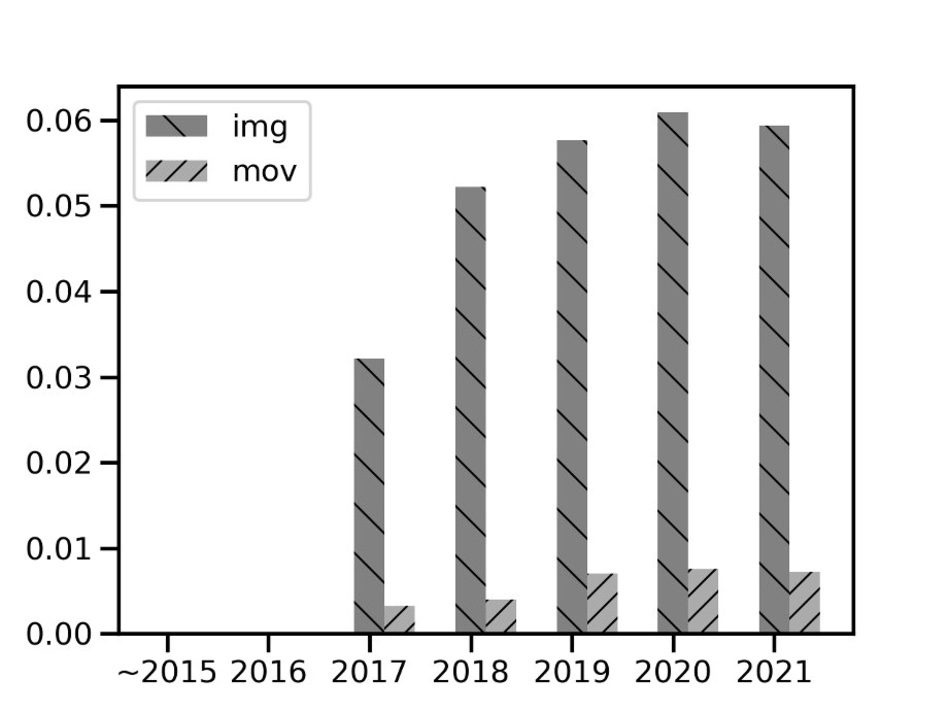
\includegraphics[width=1\linewidth]{./figures/data-category-trend.pdf}
\caption{ 
  An overview of the data collection
  }
\label{fig:data-collection-overview}
\end{figure*}


\subsection{Data Collection}
%\fig{fig:data-collection-overview} shows an overview of the data collection process. 
We first collected closed issue reports with \texttt{PyGitHub}\footnote{\url{https://pygithub.readthedocs.io/en/latest/index.html}} that internally execute GitHub API v3\footnote{\url{https://docs.github.com/en/rest}}. 
Next, we collected videos and images attached to the issue reports. While GitHub users can see videos and images on issue pages, the videos and images are stored in different URLs. As the URLs are written in the text description of issue reports, we parsed them with regular expressions and downloaded them. The regular expressions we used are shown as follows:
\begin{quote}
\addtolength\leftmargini{0in}
{\it https://user-images.githubusercontent.com/[a-zA-Z0-9\textbackslash-/]+\textbackslash.[a-zA-Z0-9]+}
\end{quote}
Each downloaded file was determined to be a image or video by its extension. Specifically, png, PNG, jpg, JPG, and jpeg are treated as images, and  gif, GIF, mp4, MP4, and mov as videos.
Consequently, we downloaded 33,079 images and 3,819 movies
with the collected URLs.\masa{to kuramoto: i wrote these numbers. are the numbers correct?} 


% \begin{table*}[h]
    \begin{center}
    \caption{Examples of the retrieved issues with the values of the attributes}
    \begin{tabular}{c c c c c c c} 
      \toprule
      \textbf{IssueCreatedYear} &
      \textbf{ResolutionTime} &
      \textbf{Images} &
      \textbf{Videos} &
      \textbf{Comments} &
      \textbf{FirstCommentTime} &
      \textbf{DescriptionLength} \\
      \midrule
      2020 & 6.99861111 & 0 & 0 & 1 & 6.99861111 & 4430\\
      2020 & 41.9594329 & 1 & 0 & 3 & 17.7784722 & 85\\
      2020 & 43.8850579 & 0 & 0 & 2 & 0.49828704 & 56\\
      2020 & 44.0935532 & 0 & 0 & 4 & 0.91277778 & 33\\
      2020 & 0.14934028 & 0 & 0 & 8 & 0.08077546 & 244\\
      2020 & 59.5670949 & 2 & 0 & 5 & 0.39472222 & 102\\
      2020 & 74.9322569 & 0 & 0 & 0 & -          & 24\\
      \bottomrule
    \end{tabular}
    \label{tab:example-dataset}
    \end{center}
  \end{table*}

% We extract a part of the retrieved issues in \tab{tab:example-dataset}. 
% Each row corresponds to the values of the attributes of an issue. 
%
\begin{table}[t]
    \begin{center}
    \caption{The attributes we collected from the issues}
    \scalebox{0.85}[0.85]{
    \begin{tabular}{ll} 
        \toprule
        \multicolumn{1}{c}{\textbf{Attributes}} & \multicolumn{1}{c}{\textbf{Description}} \\ 
        \midrule
        $IssueResolvedTime$ & The time until the issue is resolved (day) \\
        $FirstCommentTime$ & The time until the first comment (day) \\
        $\#comments$ & The number of comments \\
        $\#chars$ & \masa{im not sure what is this} \\
        $\#imgs$ & \# of attached images when the issue is created \\
        $\#movs$ & \# of attached movies when the issue is created \\
        $\#words$ &  \masa{im not sure what is this} \\
        $IssueCreatedYear$ & The year when the issue is created \\
        \bottomrule
    \end{tabular}
    }
    \label{tab:issue-attr}
    \end{center}
\end{table}


\begin{table}[t]
    \begin{center}
    \caption{The attributes we collected from the issues}
    \scalebox{0.85}[0.85]{
    \begin{tabular}{ll} 
        \toprule
        \multicolumn{1}{c}{\textbf{Attributes}} & \multicolumn{1}{c}{\textbf{Description}} \\ 
        \midrule
        $IssueResolvedTime$ & The time until the issue is resolved (day) \\
        $FirstCommentTime$ & The time until the first comment (day) \\
        $\#comments$ & The number of comments \\
        $\#chars$ & \masa{im not sure what is this} \\
        $\#imgs$ & \# of attached images when the issue is created \\
        $\#movs$ & \# of attached movies when the issue is created \\
        $\#words$ &  \masa{im not sure what is this} \\
        $IssueCreatedYear$ & The year when the issue is created \\
        \bottomrule
    \end{tabular}
    }
    \label{tab:issue-attr}
    \end{center}
\end{table}

\subsection{Analysis}
We retrieved the attributes from the collected issue reports.
\tab{tab:issue-attr} shows seven attributes extracted from 
the issue reports. 
The attributes can be classified into three dimensions, 
``Report'', ``Discussion'', and ``Fix''. 
The attributes in the dimension ``Report'' are extracted from 
the description of issue reports or attached files 
when the issue was created. 
In particular, in RQ1, we 
%calculate 
utilize the number of words 
in reports (\ie, $DescriptionLength$) for Img, Vid, and None. 
In addition,  $\#imgs$ and $\#vids$ are used to show 
dataset description. 
Note that these attributes are not calculated from either title, not comments (i.e., only descriptions were used). 
Also, when computing $DescriptionLength$, if the description of the issue report 
includes URLs for images/videos, 
we exclude them from the description because these are not words.

The dimension ``Discussion'' has two attributes, $Comments$ and $FirstCommentTime$. $Comments$ is the number of comments were made in the issue report. We utilize this attribute as a proxy measure of discussion effort. $FirstCommentTime$ is the days subtract from when the first comment was made to when issue was reported. We employ this attribute for measuring developers' interest. 

The dimension ``Fix'' has one attribute $IssueResolvedTime$ which shows the time from reported to fixed. 
Note that some negative values of $IssueResolvedTime$ were observed. We investigated it manually and found that these are because of a bug in GitHub.  We excluded those issues that have negative values from our dataset. 
In addition, we excluded issue reports resolved in too short or long periods (e.g., 30 seconds) because they might be issued after being fixed or might not be fixed in reality.
%\kashiwa{check please}
Specifically, we only use the issue reports that meet the condition: $30\ sec \leq IssueResolvedTime \leq 1\ year$.
The number of issue reports that meet this condition is 711,160 (92.23\%).


\kashiwa{Write what do you analyze (e.g., compare them in median)}
To evaluate the difference, we used a non-parametric test \textit{Steel-Dwass test}.
\kashiwa{Write what this test is}
\kashiwa{Write why this test is selected}
because our preliminary study shows that 
the distributions for each category do not 
come from normal distributions.
\kashiwa{Write the reason why correction is not needed (i.e., how to deal with family-wise error rate)}

% 調査
\section{調査}
\subsection{動画・画像の活用件数の推移}
図\ref{content_trend}は,動画及び画像の活用件数の含有率の年別推移である.
2016年までは,画像の活用は0.01\%未満であり,動画に関しては0件であった.
2017年以降,活用件数は急激に増加し,2021年には,動画~0.72\%,画像~5.93\%であった.
2017年以降に急激に増加した要因に関しては,調査中である.

\begin{figure}[t]
  \begin{center}
      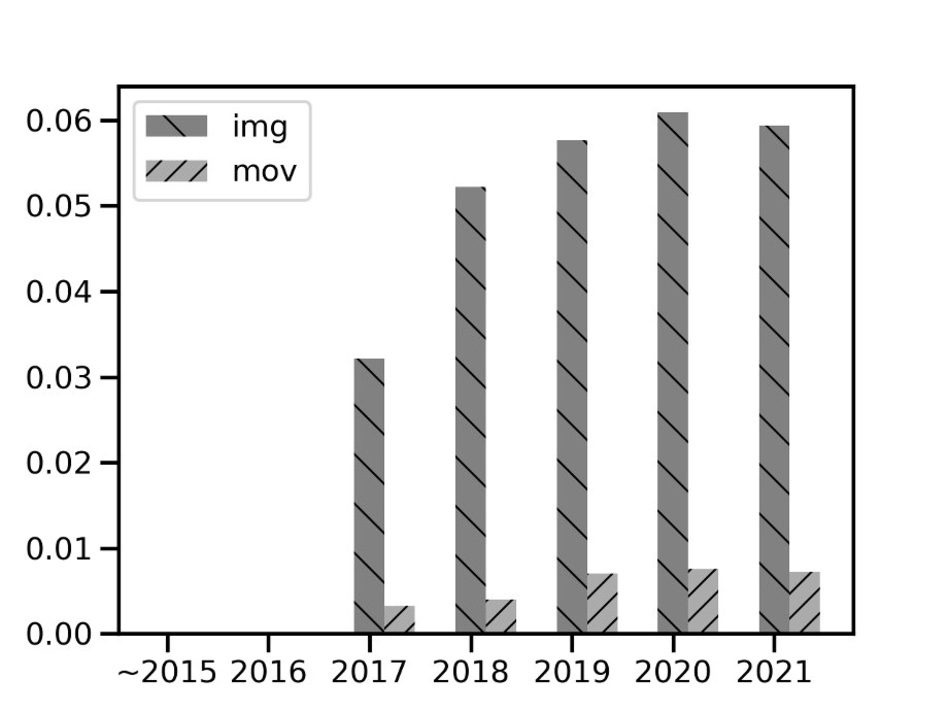
\includegraphics[scale=0.5]{./image/data_content_trends.pdf}
      \caption{動画・画像の含有率推移 \label{content_trend}}
  \end{center}
\end{figure}

\subsection{データの分析}

\begin{figure*}[t]
  \begin{center}
      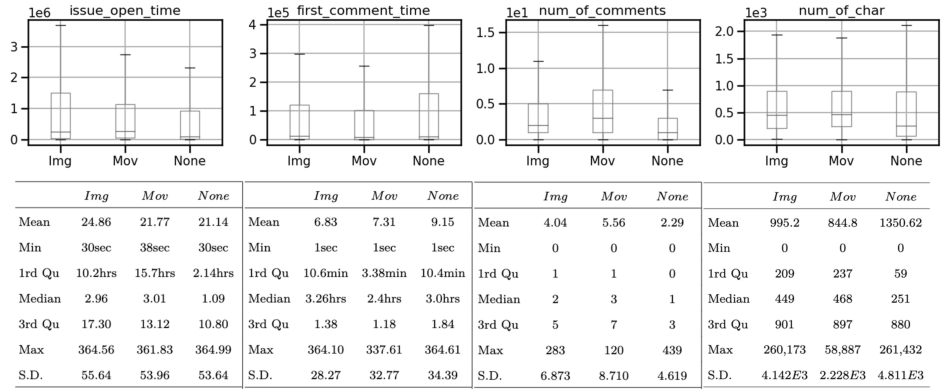
\includegraphics[scale=1.1]{./image/dataset_plot.pdf}
      \caption{Issue群ごとの調査項目の分布及び代表値 \label{dataset_plot}}
  \end{center}
\end{figure*}

図\ref{dataset_plot}は,データの特性値を箱ひげ図及び表で表現したものである.
ただし,図\ref{dataset_plot}の箱図の最大値は,$3rd~Qu + 1.5 * IQR$以下の最大値である.
($IQR$:四分位範囲)
\\
% この様な処理は,データの中央値付近を見やすくする為にしばしば用いられる.
\noindent{\bf{正規性について.}}
%図\ref{dataset_plot}では,$Issue\_open\_time$,$First\_comment\_time$及び$Num\_of\_char$の平均値が,
%四分位範囲内に収まっていないことから正規分布から逸脱している.
%$Num\_of\_comments$に関しては,正規分布しているような印象を受ける.
%実際,$Img$の平均値 = 4.04,標準偏差$S.D.$ = 6.873であり,これから$\pm~3S.D.$の上限値は24.66と算出できる.
%これから,最大値283は外れ値であるとも考えられる.しかし,
$Kolmogorov-Smirnov$検定の結果,すべての項目に対して,正規性は有意水準0.05で棄却された.
\\
\noindent{\bf{等分散性について.}}
$Leneve$検定の結果を表\ref{levene_result}に示す.
帰無仮説は「すべてのIssue群間を通して等分散」であり,有意水準は0.20とする.

\begin{table}[h]
  \begin{center}
  \caption{等分散性検定・結果}
  \begin{tabular}{l|c c} 
    \hline
     & 有意確率 & 平均分散比 \\ 
    \hline \hline
    $Issue\_open\_time$ & 0.378 & 1.050 \\
    $First\_comment\_time$ & 0.296 & 1.301 \\
    $Num\_of\_comments$ & 0.001 & 2.459 \\
    $Num\_of\_char$ & 0.073 & 3.156 \\
    \hline
  \end{tabular}
  \label{levene_result}
  \end{center}
\end{table}

$Num\_of\_comments$及び$Num\_of\_char$は,等分散性が有意水準0.20で棄却される.
$Issue\_open\_time$及び$First\_comment\_time$は,有意確率が有意水準以上であることと,
平均分散比が~1~\textasciitilde ~1.5~程度であることから,等分散性を仮定する.


\subsection{統計的検定}
本小節の目的は,群間の分布の差が統計的に有意であるかの検定である.
検定には,正規性及び等分散性を仮定しない$Steel-Dwass$法を用いる.
$Steel-Dwass$法による検定結果を表\ref{Steel-Dwass_result}に示す.
ただし,有意水準は0.05とする.

\begin{table}[t]
  \begin{center}
  \caption{調査項目ごとの多重比較の結果}
  \begin{tabular}{l r|r}
    \hline
    調査項目 & 対 & 有意確率 \\
    \hline \hline
    $Issue\_open\_time$ & & \\
     & \bf{$Img$~vs~$None$} & **~0.002 \\
     & \bf{$Mov$~vs~$None$} & **~0.021 \\
     & \bf{$Img$~vs~$~Mov$} & 0.381 \\
    \hline
    $First\_comment\_time$ & & \\
     & \bf{$Img$~vs~$None$} & 0.764 \\
     & \bf{$Mov$~vs~$None$} & 0.351 \\
     & \bf{$Img$~vs~$~Mov$} & 0.404 \\
    \hline
    $Num\_of\_comments$ & & \\
     & \bf{$Img$~vs~$None$} & *~0.001 \\
     & \bf{$Mov$~vs~$None$} & *~0.001 \\
     & \bf{$Img$~vs~$~Mov$} & 0.211 \\
    \hline
    $Num\_of\_char$ & & \\
     & \bf{$Img$~vs~$None$} & *~0.001 \\
     & \bf{$Mov$~vs~$None$} & *~0.001 \\
     & \bf{$Img$~vs~$~Mov$} & 0.599 \\
    \hline
  \end{tabular}\\
  \small
    *~ : 両側検定で有意 ~~~ ** : 片側検定で有意\\
  \label{Steel-Dwass_result}
  \end{center}
\end{table}

$Img$及び$Mov$は,$None$に比べて,$Issue\_open\_time$が有意に大きく,
$Num\_of\_comments$及び$Num\_of\_char$については分布に何らかの有意な差があると解釈できる.
一方で,$First\_comment\_time$においては,有意差は認められなかった.
また,$Img$と$Mov$の比較では,すべての項目で有意差は認められなかった.
有意差が認められなかった項目については,有意差の有無は判断を保留する.

\subsection{出現単語分析}
Issueのテキストに含まれる単語を\textbf{tf\_idf}値に変換し,同じIssue群に属すもの同士をマージした結果,\textbf{tf\_idf}値が大きい順に10個の結果を表\ref{tf-idf_result}に示す.
"at"や"it","the"などの単語を除外する為,
名詞,動詞及び疑問詞のみを対象とした. \\

\begin{table}[t]
  \begin{center}
  \caption{Issue群ごとの\textbf{tf\_idf}上位10単語}
  \begin{tabular}{r | c c c }
     & $Img$ & $Mov$ & $None$\\
    \hline \hline
    1 & image & when & dependabot\\
    2 & screenshot & dropdown & code\\
    3 & when & view & file\\
    4 & error & package & pullrequest\\
    5 & screen & issue & version\\
    6 & version & python & error\\
    7 & shot & height & use\\
    8 & file & react & lib\\
    9 & test & button & add\\
    10& code & text & commit\\
  \end{tabular}\\
  \label{tf-idf_result}
  \end{center}
\end{table}
% 考察
\section{結果と考察\label{research}}

画像及び動画を含むIssueは,そうでないIssueに比べて,
$Issue\_open\_time$が平均で,2.9\%\textasciitilde17.6\%増加し,
$Num\_of\_comments$が平均で76.4\%\textasciitilde143\%増加した.
一方で,$First\_comment\_time$が平均で20.1\%\textasciitilde25.4\%減少し,
$Num\_of\_char$が平均で26.3\%\textasciitilde 37.5\%減少した.
$Issue\_open\_time$及び$Num\_of\_comments$が増加していることから,
動画及び画像は,比較的難しい問題に対して用いられているのではないかと推察される.

\begin{itembox}{動画及び画像による効果及び傾向}
  ・状況報告を細かく記述せずに済む\\
  ・開発者の問題への着手を早める\\
  ・コメントが得やすくなる\\
  ・難しい問題に用いられやすい
\end{itembox}

また,$Img$と$Mov$の間では,どの項目においても有意な差は認められなかったことから,
動画と画像のどちらを用いるかよりも,用いるか用いないかが重要であると推察される.

出現単語分析では,$Img$では表示に関係する単語が多く,
$Mov$では"dropdown","button"及び"react"など動きのある画面に関する単語が多い印象を受ける.
一方で,$None$では,コーディングに関する単語が多い結果であった.
$Mov$では"when"が1番目に,$Img$でも3番目にランクインした.これは,不具合の再現方法に関する記述である可能性が高い.
実際,目視調査で,不具合の再現動画が多いことを実験的に確かめた.
一方で,$None$では1番目に"dependabot"がランクインした.DependaBotは,最新のライブラリを推奨したり更新するボットであり,
設定により自動でIssueを生成することもある.
$Img$及び$Mov$と$None$の差は,ボットによる影響を受けている可能性がある.

\begin{itembox}{動画及び画像を用いられやすい場面}
  ・不具合が画面に関する場合に画像\\
  ・画面の動きに関する場合に動画
\end{itembox}


一般にサンプルサイズは多ければ多いほど,母集団の特徴をより正確に抽出できる.
ところが検定においては,サンプルサイズが大きくなるにつれて,誤差に過剰に反応し,有意確率が小さくなる傾向がある.
すまわち,検定で有意差を得たとしても,母集団分布の有意な差によるものか,サンプルサイズが大きすぎることによるものか判断できないのである.
従って,適切なサンプルサイズを前もって決めておくことが重要である.
本調査では,事前に効果量の目安が得られなかったために,やや恣意的に決定した.
検定結果を見ると,有意差がはっきりと認められた部分と,認められなかった部分が見られた$Issue\_open\_time$,$Num\_of\_comments$及び$Num\_of\_char$に対しては適切なサンプルサイズであったと推察する.
一方で$First\_comment\_time$に対しては,実際に有意と言える差が無いか,あるいは,サンプルサイズが小さすぎた可能性がある.

また本調査では,すべての調査項目が正規分布に従わなかった.
一般に,正規分布を仮定しない検定法よりも,正規分布を仮定する検定法は検出力に長けていると言われている.
従って,データが正規分布に従わない場合,正規分布に近似するため適切な変数変換を行う.
時系列データの変換には対数変換が多くの場合有効である.本調査の調査項目の一部は時系列データであり,
変換が推奨される場面であるが,実際に適用させたところ平均値の群間順序関係が変化したことと,
順位和検定により順位に変換されることから,対数変換を用いずに調査した.
% 妥当性への脅威
\section{妥当性への脅威\label{threats}}

%\noindent{\bf 内的妥当性.}

\noindent{\textbf{内的妥当性.}}本調査で用いた等分散性の検定の有意水準について,留意しなければならない点がある.
多重比較法は等分散性に関して,二群比較よりも鋭敏であり,有意水準0.20程度で行わなければ意味をなさないことが示されている.\cite{Test_Level}
さらには,有意水準0.50まで引き上げても,誤った結果を招く場合があると言われている.
その場合,$Issue\_open\_time$及び$First\_comment\_time$の等分散性は棄却され,
「動画及び画像があるIssueは,そうでないものに比べて$Issue\_open\_time$が有意に大きい」とした表現は,
「動画及び画像があるIssueは,そうでないものに比べて$Issue\_open\_time$に何らかの有意な差をもたらす」となる.

また,ボットが$None$に多くあらわれていることが,出現単語分析で明らかになった.
botを取り除く処理をしなければ,分布差が動画及び画像によるものとは断定できない.その点が考慮されていない.

Issueで報告される内容は,不具合に関するものだけではない.
事前調査では,新たな機能の提案に関する報告があることも確認した.
ただこの場合に関しても,動画及び画像により提案者の意図が伝わりやすくなることは,
バグの症状理解が早まることと本質的に同じと考えている.

また,本調査はデータマイニングに十分な期間を確保できなかった為,マイニングしたリポジトリは全体の2\%以下と少ない.
より正確な結果を得るために,マイニング量を増やすことは今後の課題である.

\noindent{\textbf{外的妥当性.}}
本調査の調査対象は,条件に適合したリポジトリのみであり,すべての開発現場で同様の傾向があるとは限らない.
また,開発規模や分野など,リポジトリの性質が考慮されていない.
% まとめと今後の展望
\section{Conclusion}
\label{sec:conclusion}

\masa{conclusion here}

Finally, we present future research directions with our dataset. 


\noindent
\textbf{The impact analysis of movies and images on software development.}
GitHub added the feature~\citep{github-video-blog} to easily 
share movies with GitHub to earn advantages 
in software development such as reproducing bugs easily in issues and 
explaining the background of changes in pull requests. 
However, no studies exist that investigate whether such movies 
impact software development. 
Hence, investigating the impact of movies on software development 
is a future research direction. 
Specifically, we study the reduction of issue resolution time, 
the response rate of developers, and 
the reduction of the number of comments 
in which developers write ``works for me''. 

\noindent
\textbf{Automated bug reproduction with image processing.}
Reproducing bugs is a time-consuming process 
in software development\masa{citation}.
Automating this process would support developers 
to quickly find and fix the cause of bugs. 
Hence, it is an important future research direction 
to automate bug reproduction. 
As the evolution of image processing with deep learning models, 
the accuracy of image processing significantly improves\masa{citation}. 
Hence, we apply such deep learning models to movies 
to implement automated bug reproduction tools. 
}

\section*{謝辞}
本研究の一部はXXXの助成を受けた.

%\bibliographystyle{jplain}
%\bibliography{references}

\bibliographystyle{junsrt}
\bibliography{references}
%\begin{thebibliography}{9}% 文献数が10未満の時 {9} 10以上の時は{99}
%    \bibitem{}
%\end{thebibliography}

\end{document}
